\chapter{Implementazione} \hypertarget{cleancode}{} \hypertarget{chiara2}{}
\label{cap:progettazione-codifica}

\lstset{
    escapeinside={(*@}{@*)}, % Delimitatori per modalità LaTeX
    basicstyle=\ttfamily,    % Stile monospaziato
}

\intro{Di seguto viene decritto il processo implementativo. In particolare la classe \emph{GA} che modella l'algoritmo genetico e \emph{Chromosome} che facilita la manipolazione dei cromosomi all'interno di \emph{GA}. Sono state utilizzate procedure interne come \emph{PlacementHeuristicEPs} e \emph{PlacementHeuristicEPs\_with\_pilot\_method}, che utilizzano le metriche \emph{CONTACT\_PERIMETER}, \emph{PILOT\_METHOD} e \emph{AREA\_DESCENDING} [\hyperlink{bibliografia}{5}].
Per rendere il codice più pulito, mantenibile e comprensibile, sono state usate le linee guida espresse in \textbf{Clean Code} [\hyperlink{bibliografia}{6}]} 

\section{Classe \emph{chromosome}}

La classe \emph{Chromosome} modella un cromosoma, ovvero una possibile soluzione, in una struttura dati che incapsula una sequenza di geni (ovvero gli \emph{Item}, o elementi) e il relativo valore di fitness, grado di adeguatezza del cromosoma al problema. La classe è progettata per essere versatile, con metodi che facilitano la manipolazione e l'evoluzione di cromosomi durante l'esecuzione dell'algoritmo.

La classe \textbf{Item} rappresenta un elemento \( i \in E_O\) o \( j \in E_P\) posizionabile su un foglio \( t \in T \). Ogni elemento è caratterizzato da un identificativo univoco e da un tipo che ne determina proprietà fisiche come larghezza, altezza, margini e altre specifiche geometriche.

Le dimensioni e la posizione dell'oggetto sono definite da attributi come larghezza, altezza, la coordinata del punto superiore sinistro, e l'angolo di rotazione, che può assumere valori predefiniti (0°, 90°, 180°, 270°). Vengono calcolate dinamicamente proprietà come area e perimetro, utili per ottimizzazioni, e sono gestite le rotazioni consentite per ogni oggetto. Inoltre, include vincoli di precedenza, sia \emph{hard} che \emph{soft}, che regolano l'ordine in cui può essere posizionato.

\subsection{Attributi}

\begin{itemize}
    \item \textbf{\texttt{genes}}:
    \begin{itemize}
        \item \textbf{Tipo}: Lista
        \item \textbf{Descrizione}: Contiene la sequenza di geni che rappresenta la soluzione codificata. I geni vengono costruiti all'inizio del processo di generazione della popolazione iniziale all'interno del genetico, utilizzando i parametri di input \emph{items} e \emph{optionals}, che corrispondono agli elementi obbligatori \( E_O \) e opzionali \( E_P \) di un istanza. \emph{items} e \emph{optionals} sono codificati come una sequenza \emph{Item}.
    \end{itemize}
    \item \textbf{\texttt{fitness}}:
    \begin{itemize}
        \item \textbf{Tipo}: Float
        \item \textbf{Descrizione}: Valore che rappresenta la qualità della soluzione codificata dal cromosoma. Questo valore è calcolato da una funzione di fitness definita all'interno dell'algoritmo genetico.
    \end{itemize}
    \item \textbf{\texttt{pilot\_method}}:
    \begin{itemize}
        \item \textbf{Tipo}: Booleano
        \item \textbf{Descrizione}: Flag che può essere utilizzato per scegliere quale tipo di \emph{decode} utilizzare. In seguto verrà descritta la differenza fra i due tipi di \emph{decode}.
    \end{itemize}
\end{itemize}

\subsection{Metodi}

\begin{itemize}
    \item \textbf{Costruttore: \texttt{\_\_init\_\_(self, genes)}}
    \begin{itemize}
        \item Inizializza un oggetto \emph{Chromosome} con una lista di geni fornita come argomento.
        \item Imposta inizialmente il valore di fitness a \emph{None} e \emph{pilot\_method} a \emph{False}.
    \end{itemize}

%     \begin{lstlisting}[language=Python]
% def __init__(self, genes):
%     self.genes = genes
%     self.fitness = None
%     self.pilot_method = False
%     \end{lstlisting}

    % \item \textbf{Lunghezza: \texttt{\_\_len\_\_(self)}}
    % \begin{itemize}
    %     \item Restituisce il numero di geni contenuti nel cromosoma.
    %     \item Utile per valutare la dimensione del cromosoma durante le operazioni genetiche come la mutazione o il crossover.
    % \end{itemize}

%     \begin{lstlisting}[language=Python]
% def __len__(self):
%     return len(self.genes)
%     \end{lstlisting}

    \item \textbf{Accesso agli elementi: \texttt{\_\_getitem\_\_(self, idx)}}
    \begin{itemize}
        \item Permette l'accesso diretto a un gene tramite l'indice \emph{idx}, come se il cromosoma fosse una lista.
    \end{itemize}

%     \begin{lstlisting}[language=Python]
% def __getitem__(self, idx):
%     return self.genes[idx]
%     \end{lstlisting}

    % \item \textbf{Confronto di uguaglianza: \texttt{\_\_eq\_\_(self, other)}}
    % \begin{itemize}
    %     \item Confronta due cromosomi per verificarne l'uguaglianza in base ai geni, alla fitness e al flag \emph{pilot\_method}.
    % \end{itemize}

%     \begin{lstlisting}[language=Python]
% def __eq__(self, other):
%     if isinstance(other, Chromosome):
%         return self.genes == other.genes and self.fitness == other.fitness and self.pilot_method == other.pilot_method
%     return False
%     \end{lstlisting}

    % \item \textbf{Copia: \texttt{copy(self)}}
    % \begin{itemize}
    %     \item Crea e restituisce una copia indipendente del cromosoma, copiando sia i geni che \emph{fitness} e \emph{pilot\_method}.
    % \end{itemize}

%     \begin{lstlisting}[language=Python]
% def copy(self):
%     ch = Chromosome(self.genes[:])
%     ch.fitness = self.fitness
%     ch.pilot_method = self.pilot_method
%     return ch
%     \end{lstlisting}

    \item \textbf{Aggiornamento della fitness: \texttt{update\_fitness(self, ga\_instance)}}
    \begin{itemize}
        \item Aggiorna il valore del fitness del cromosoma utilizzando una funzione di fitness definita all'interno di un'istanza dell'algoritmo genetico (\emph{ga\_instance}).
    \end{itemize}

%     \begin{lstlisting}[language=Python]
% def update_fitness(self, ga_instance):
%     self.fitness = ga_instance.fitness(self)
%     \end{lstlisting}

    \item \textbf{Ordinamento prioritario: \texttt{priority\_sort(self)}}
    \begin{itemize}
        \item Ordina i geni del cromosoma in base a una funzione lambda che utilizza attributi specifici di ciascun gene, ovvero \emph{precedence} e \emph{soft\_precedence}, interi che indicano rispettivamente il grado di precedenza obbligatoria e opzionale. In particolare, 0 indica l'assenza di un vincolo di precedenza, 1 la precedenza massima e a seguire diminuisce il grado di precedenza.
        \item Questo metodo è fondamentale poiché è necessario mantenere sempre un ordinamento prioritario all'interno dei geni di un cromosoma.
    \end{itemize}

%     \begin{lstlisting}[language=Python]
% def priority_sort(self):
%     self.genes = sorted(self.genes, key=lambda item: (item.precedence, item.soft_precedence))
%     \end{lstlisting}
    \item Sono presenti anche altri metodi utili per semplificare lo sviluppo degli operatori genetici, come: operatore di uguaglianza, metodo per creare una copia del cromosoma e metodo per restituire la lunghezza del cromooma.
\end{itemize}

\subsection{Ruolo della classe nell'algoritmo genetico}

La classe \emph{Chromosome} è progettata per essere una componente centrale di un algoritmo genetico, con le seguenti funzionalità principali:
\begin{itemize}
    \item \textbf{Codifica delle soluzioni}: I geni rappresentano gli \emph{item} o elementi;
    \item \textbf{Calcolo del fitness}: L'attributo \emph{fitness} consente di valutare la qualità del cromosoma in relazione all'obiettivo del problema;
    \item \textbf{Evoluzione}: La classe facilita operazioni come crossover, mutazione e selezione grazie alla possibilità di accedere e modificare i geni;
    \item \textbf{Flessibilità}: L'uso di attributi aggiuntivi come \emph{pilot\_method} rende la classe adattabile a diversi scenari e metodi euristici.
\end{itemize}

\section{Classe GA}

La classe \textbf{GA} è progettata per essere modulare e configurabile, grazie alla sua capacità di accettare diversi parametri di configurazione tramite l'oggetto \emph{conf}. Questi parametri includono:
\begin{itemize}
    \item \textbf{Dimensione della popolazione}: il numero totale di individui nella popolazione;
    \item \textbf{Probabilità di crossover e mutazione}: definiscono la frequenza con cui avvengono questi eventi;
    \item \textbf{Pool di selezione}: definisce gli individui a cui verranno applicati gli operatori genetici;
    \item \textbf{Elitismo}: quantità di individui migliori da trasmettere direttamente alla generazione successiva;
    \item \textbf{Limite di tempo}: specifica quanto a lungo il processo evolutivo può continuare.
\end{itemize}

\subsection{Costruttore}
Il costruttore della classe definisce e inizializza tutti gli attributi necessari per il funzionamento dell'algoritmo genetico.

% Sono inclusi vincoli di posizionamento sotto forma di aree proibite e forzate, definite per ciascun lato (sinistra, destra, sopra e sotto). Questi vincoli determinano le zone dove la parte non può o deve essere posizionata. Margini aggiuntivi, specifici della parte o del formato del foglio, vengono utilizzati per garantire separazioni o tolleranze durante il posizionamento.

Di seguito analizziamo i parametri passati in input e il loro ruolo.

\begin{itemize}
    \item \emph{conf}: Oggetto che contiene la configurazione dell'algoritmo genetico (dimensione della popolazione, probabilità di crossover e mutazione, dimensione dell'élite, limite di tempo). Questo oggetto fornisce i parametri chiave per il controllo dell'evoluzione.
    \item \emph{items} e \emph{optionals}: Liste di oggetti \emph{Item} rappresentanti elementi da ottimizzare. \emph{items} rappresenta gli elementi obbligatori \(E_O\), mentre \emph{optionals} rappresenta quelli opzionali \(E_P\).
    \item \emph{sheet} è un oggetto della classe \textbf{Sheet} che rappresenta un foglio \(T\) utilizzato come superficie per posizionare oggetti in processi di ottimizzazione spaziale come il nesting. Ogni foglio è caratterizzato da un tipo specifico che ne definisce le proprietà fisiche e geometriche, come larghezza, altezza e spessore. Oltre alle dimensioni, la classe gestisce i margini specifici per ogni lato del foglio, utilizzati per definire aree sicure per il posizionamento degli oggetti. 
    \item \emph{formats} indica la quantità e le dimensioni disponibili per i fogli.
    \item \emph{parts} è una lista di oggetti di classe \textbf{Part}. Questa classe modella un componente (o elemento) da posizionare in un foglio \emph{sheet}. Ogni istanza rappresenta una parte con caratteristiche fisiche, restrizioni geometriche e proprietà che influenzano il posizionamento. Ogni parte ha un identificativo univoco, un ID descrittivo, e una quantità che indica il numero di istanze richieste. La classe gestisce priorità di posizionamento tramite un parametro di precedenza, utilizzabile per stabilire un ordine preferenziale. Inoltre, supporta diverse configurazioni di rotazione, consentendo di specificare se la parte può essere ruotata a 0°, 90°, 180° o 270°, per adattarsi meglio al contesto del foglio.
    \item \emph{eval\_criterion}: Criterio di valutazione usato per calcolare la fitness degli individui. Nel caso specifico, viene utilizzato il \emph{CONTACT\_PERIMETER} che calcola la quantità di perimetro di un oggetto che entra in contatto con i bordi di un foglio, o con altri oggetti già posizionati, per sceglierne il posizionamento migliore, in caso di pareggio mette sempre l'oggetto in orizzontale (in base al lato più lungo).
    \item \emph{pilot\_method\_prob}: Probabilità di applicare il criterio di valutazione denominato \emph{PILOT\_METHOD} (invece del il \emph{CONTACT\_PERIMETER}) per valutare la fitness di una soluzione. Questo criterio valuta la quantità di scarto (area inutilizzata) generata dal posizionamento di un insieme di oggetti su un foglio.
    \item \emph{is\_precedence\_hard}: Flag che determina se i vincoli di precedenza sono rigidi o meno.
    \item \emph{sorting\_criteria}: Criteri di ordinamento per la generazione iniziale della popolazione, in questo caso \emph{AREA\_DESCENDING}, ovvero ordine di grandezza in base all'area, dall'\emph{Item} con l'area maggio a quello con l'area minore.
\end{itemize}

\subsection{Generazione della popolazione iniziale}

La popolazione iniziale è generata combinando un criterio di ordinamento specifico e un processo di perturbazione. I passi principali sono:

\begin{itemize}
    \item \textbf{Criterio di Ordinamento}: Gli elementi sono ordinati in base al criterio \emph{AREA\_DESCENDING}, che privilegia gli elementi con area maggiore. Questo approccio mira a massimizzare l'uso dello spazio disponibile nei fogli;
    \item \textbf{Perturbazione}: A partire dagli elementi ordinati, una porzione della popolazione subisce una ``perturbazione'' attraverso una mutazione controllata (applicata un numero di volte pari al 30\% del numero di geni per ogni cromosoma). Questo introduce diversità nella popolazione e riduce la probabilità che l'algoritmo converga prematuramente.
\end{itemize}

La generazione iniziale è cruciale per garantire che la popolazione esplori efficacemente il panorama delle possibili soluzioni.

\subsection{Gestione del flag \emph{pilot\_method}}
Il flag \texttt{pilot\_method} è un elemento innovativo dell'algoritmo, infatti, in letteratura non sono diffusi algoritmi genetici con doppio \emph{decode}:

\begin{itemize}
    \item \textbf{Assegnazione Iniziale}: Una porzione della popolazione iniziale è selezionata casualmente per essere decodifica con il criterio di valutazione \emph{PILOT\_METHOD}. La probabilità di assegnazione è controllata dal parametro \emph{pilot\_method\_prob};
    \item \textbf{Effetto sul Processo}: Il \emph{PILOT\_METHOD} modifica il comportamento degli individui durante la fase di decodifica. È progettato per gestire situazioni di conflitto o pareggio (\emph{tie-breaking}) nelle soluzioni. Si è resa necessaria una doppia decodifica per bilanciare l'efficienza del \emph{CONTACT\_PERIMETER} con il \emph{tie-break} molto più profondo del \emph{PILOT\_METHOD};
    \item \textbf{Ereditarietà e Mutazione}: Durante la riproduzione, il flag può essere trasferito ai figli. Inoltre, una mutazione del flag può alterare la probabilità che un individuo utilizzi il metodo \emph{PILOT\_METHOD};
    \item \textbf{Limitazioni}: Un limite massimo alla dimensione della popolazione con il flag \emph{pilot\_method} è imposto per ridurre il costo computazionale.
\end{itemize}

\subsection{Riproduzione e rimpiazzo}

La riproduzione si basa su operatori genetici fondamentali di selezione, crossover e mutazione, per generare l'\emph{offspring} (popolazione di figli) mentre la strategia di rimpiazzo combina gli individui della popolazione corrente e l'\emph{offspring} generato per formare la nuova popolazione. Gli individui migliori della popolazione attuale sono preservati, mentre, i figli con fitness più elevato (esclusi quelli con flag \emph{pilot\_method} oltre il limite) vengono inclusi per rimpiazzare il resto della popolazione. Questa strategia garantisce un equilibrio tra diversificazione e intensificazione.

\subsection{Funzione di fitness con doppio decoding}

La fitness di un cromosoma è calcolata come segue:

\begin{enumerate}
    \item \textbf{Doppio decode}:
    \begin{itemize}
        \item Se il flag \emph{pilot\_method} è attivo, viene utilizzato un algoritmo euristico avanzato (\emph{PlacementHeuristicEPs\_with\_pilot\_method}) per posizionare gli elementi nei fogli, risolvendo eventuali conflitti;
        \item Altrimenti, viene usato un approccio più semplice (\emph{PlacementHeuristicEPs}).
    \end{itemize}
    \item \textbf{Calcolo dello Scarto}:
    Poiché il decode viene applicato riempiendo un foglio alla volta finché non vengono esauriti gli elementi da posizionare, il calcolo dello scarto totale avviene calcolando per ogni foglio, l'area del foglio meno l'area degli elementi posizionati in esso.
    \item \textbf{Fitness Finale}:
    \[
    \text{Fitness} = \frac{\text{Area dei Fogli Utilizzati} - \text{Scarto Totale}}{\text{Area Totale Disponibile}}
    \]
\end{enumerate}

\subsection{Placement}

Le funzioni \emph{PlacementHeuristicEPs\_with\_pilot\_method} e \emph{PlacementHeuristicEPs} rappresentano due varianti di algoritmi di posizionamento di oggetti su un foglio, utilizzando il concetto di punti estremi (\emph{Extreme Points} - EPs). Entrambi gli algoritmi cercano di ottimizzare la disposizione degli oggetti rispettando vincoli di precedenza, aree disponibili e criteri di valutazione. La principale differenza tra i due è l'uso del criterio di valutazione \emph{PILOT\_METHOD} nella prima funzione per risolvere situazioni di parità nella disposizione di un oggetto. Di seguito, una descrizione dettagliata del loro funzionamento.

Ogni oggetto è testato in tutte le sue rotazioni ammesse. Per ciascuna rotazione:
\begin{itemize}
    \item Si recuperano i punti estremi disponibili e si valutano, in base a:
    \begin{itemize}
        \item \textbf{Verifica geometrica}: Controlla se l'oggetto non esce dai limiti del foglio;
        \item \textbf{Non sovrapposizione}: Verifica che l'oggetto non si sovrapponga ad altri;
        \item \textbf{Margini di sicurezza}: Assicura che ci sia un margine di sicurezza tra l'oggetto e i bordi o altri oggetti;
        \item \textbf{Valutazione}: Calcola un punteggio per la combinazione (punto estremo, rotazione).
    \end{itemize}
    \item \textbf{Risoluzione delle parità}:
    \begin{itemize}
        \item \emph{PlacementHeuristicEPs\_with\_pilot\_method}: Se più combinazioni (EP e rotazioni) hanno lo stesso punteggio migliore, viene applicato il \emph{PILOT\_METHOD}, che simula l'aggiunta temporanea di ogni oggetto (fino a riempire il foglio) e valuta l'area di scarto. Successivamente viene scelta la configurazione con il minimo scarto;
        \item \emph{PlacementHeuristicEPs}: Invece di usare il \emph{PILOT\_METHOD}, la funzione sceglie direttamente la configurazione con il punteggio migliore. Se esistono più configurazioni con lo stesso punteggio, viene scelta la prima incontrata.
    \end{itemize}
    \item L'oggetto viene posizionato nel miglior punto estremo trovato.
\end{itemize}

\subsection{Nest della soluzione finale}

Grazie alla funzione \emph{get\_best\_solution} viene estratto il cromosoma con la fitness migliore al termine del processo evolutivo. Successivamente, la funzione \emph{nest\_solution} fornisce la soluzione finale, ottimizzata e pronta per essere applicata:

\begin{itemize}
    \item Gli elementi vengono posizionati nei fogli disponibili, rispettando i vincoli specifici.
    \item Gli elementi già posizionati vengono rimossi iterativamente fino a quando non ne restano altri.
    \item La soluzione finale è rappresentata come un oggetto \emph{Nest}, che include i fogli usati, le parti posizionate e la loro disposizione.
\end{itemize}

La Figura 5.7 mostra il grafico di una soluzione a cui è applicata la funzione \emph{nest\_solution}.

\begin{figure}[!ht] 
    \centering 
    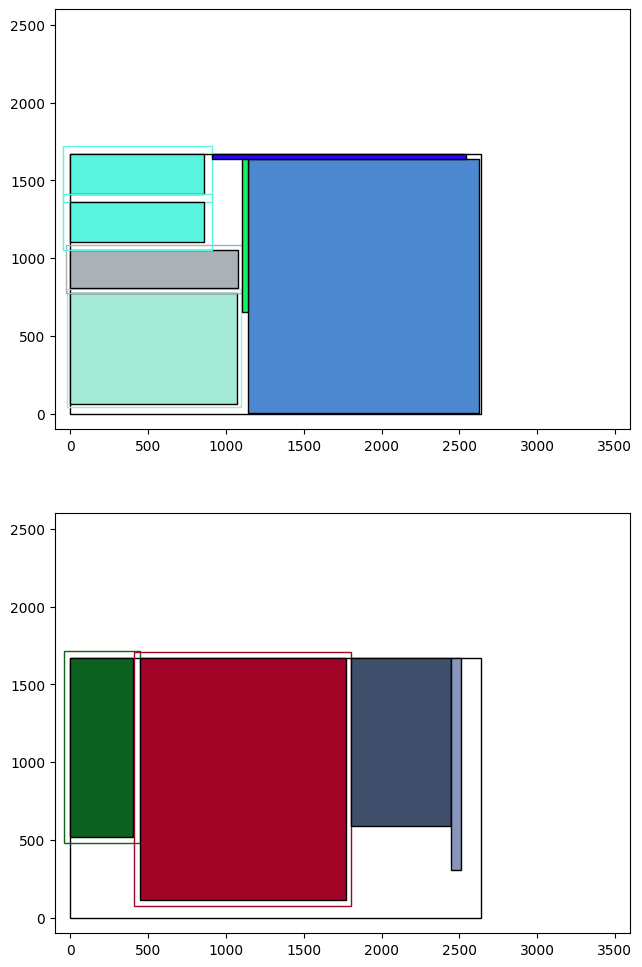
\includegraphics[width=1\columnwidth]{tesi/output} 
    \caption{Esempio nest di una soluzione}
\end{figure}




% \intro{Breve introduzione al capitolo}\\

% \section{Tecnologie e strumenti}
% \label{sec:tecnologie-strumenti}

% Di seguito viene data una panoramica delle tecnologie e strumenti utilizzati.

% \subsection*{Tecnologia 1}
% Descrizione Tecnologia 1.

% \subsection*{Tecnologia 2}
% Descrizione Tecnologia 2

% \section{Ciclo di vita del software}
% \label{sec:ciclo-vita-software}

% \section{Progettazione}
% \label{sec:progettazione}

% \subsubsection{Namespace 1} %**************************
% Descrizione namespace 1.

% \begin{namespacedesc}
%     \classdesc{Classe 1}{Descrizione classe 1}
%     \classdesc{Classe 2}{Descrizione classe 2}
% \end{namespacedesc}


% \section{Design Pattern utilizzati}

% \section{Codifica}
